
% =========================== Main File =========================== %
%							by Felix Strobel
%							Licence: CC-BY-CA
%			made for Munich University of Applied Sciences
%
% =========================== Main File ===========================

% =========================== Contribution ===========================
%						  You have found a bug?
%					Do you know a better solution?
%					  You want to add a feature?
%
%					   Then follow these steps:
%			Fork https://github.com/worldpotato/LaTeX-Template
%						  Make your changes
%				   Create a well described Pull Request
% =========================== Contribution =========================== %
% Packages
% Document class
\documentclass[
	draft=false, % shows little squares at the end of a overfull line. In case with incompatibility with other packages use: overfullrule=true to show these lines.
	twoside, % oneside or twoside
	a4paper, % din a4 format
	titlepage=firstiscover, % first page is a cover
	headsepline=true, % line between header and text
	footsepline=false, % line between text and footer number
	fontsize=12pt, % font size
	parskip=false, % adds a space at the beginning of a line after \par
	footnotes=nomultiple, % mulitiple or nomultiple, manages the devider between two footnote numbers, multiple doesn't work with hyperref
]{scrreprt}

% Remove all end-of-counter dots
\renewcommand{\autodot}{}

% for labeling list
\setkomafont{labelinglabel}{\bfseries\sffamily}
\setkomafont{labelingseparator}{\normalfont}

% to work with pictures
\usepackage{graphicx}
\graphicspath{{./img/}}
\DeclareGraphicsExtensions{.pdf,.png,.jpg} % prio1 = pdf, prio2 = png

% to wrap figures with text
\usepackage{wrapfig}

% Documentinformations
% Hyperlink creations and PDF Informations
\usepackage[
	draft=false,
	colorlinks=true, % use colors instead of frames
	linkcolor=black,
	citecolor=black,
	filecolor=black,
	menucolor=black,
	runcolor=black,
	urlcolor=black,
]{hyperref}

% For a good german
\usepackage[utf8]{inputenc}
\usepackage[english]{babel} % or german

% Bibliography
\bibliographystyle{ieeetr}

% for better looking paragraphs
% more infos at: http://www.khirevich.com/latex/microtype/
\usepackage[
	activate={true,nocompatibility}, % activate={true,nocompatibility} - activate protrusion and expansion
	final, % final - enable microtype; use "draft" to disable
	tracking=true, % tracking=true, kerning=true, spacing=true - activate these techniques
	kerning=true,
	spacing=false,
	factor=1100, % factor=1100 - add 10% to the protrusion amount (default is 1000)
	stretch=10, % stretch=10, shrink=10 - reduce stretchability/shrinkability (default is 20/20)
	shrink=10
]
	{microtype}


% for better math and more symbols
\usepackage{amsmath}
\usepackage{amssymb}
\usepackage[version-1-compatibility]{siunitx} % compatibility because you will find a lot of v1 hints with google

% to avoid some error because siunitx uses it's own fonts
\usepackage{textcomp}

% for source code
\usepackage{listings}
\usepackage{color}


\definecolor{mygreen}{rgb}{0,0.6,0}
\definecolor{mygray}{rgb}{0.5,0.5,0.5}
\definecolor{myCodeBackground}{rgb}{0.98,0.98,0.98}
\definecolor{mymauve}{rgb}{0.58,0,0.82}
\definecolor{myAmethyst}{rgb}{0.6, 0.4, 0.8}
\definecolor{myCadmiumOrange}{rgb}{0.93, 0.53, 0.18}

\lstset{
backgroundcolor=\color{myCodeBackground},% choose the background color; you must add \usepackage{color} or \usepackage{xcolor}; should come as last argument
basicstyle=\footnotesize\ttfamily, % the size of the fonts that are used for the code
breakatwhitespace=false,         % sets if automatic breaks should only happen at whitespace
breaklines=true,                 % sets automatic line breaking
captionpos=b,                    % sets the caption-position to bottom
deletekeywords={},            % if you want to delete keywords from the given language
escapeinside={\%<LaTeX>}{</LaTeX>},          % if you want to add LaTeX within your code
extendedchars=true,              % lets you use non-ASCII characters; for 8-bits encodings only, does not work with UTF-8
firstnumber=1,                % start line enumeration with line 1000
frame=none,                   % adds a frame around the code
keepspaces=true,                 % keeps spaces in text, useful for keeping indentation of code (possibly needs columns=flexible)
language=C++,                 % the language of the code
numbers=left,                    % where to put the line-numbers; possible values are (none, left, right)
numbersep=5pt,                   % how far the line-numbers are from the code
rulecolor=\color{green},         % if not set, the frame-color may be changed on line-breaks within not-black text (e.g. comments (green here))
showspaces=false,                % show spaces everywhere adding particular underscores; it overrides 'showstringspaces'
showstringspaces=false,          % underline spaces within strings only
showtabs=false,                  % show tabs within strings adding particular underscores
stepnumber=2,                    % the step between two line-numbers. If it's 1, each line will be numbered
tabsize=2,                  % sets default tabsize to 2 spaces
title=\lstname,                   % show the filename of files included with \lstinputlisting; also try caption instead of title
keywordstyle=\bfseries\color{mygreen},       % keyword style
morekeywords={*,\ldots},            % if you want to add more keywords to the set
numberstyle=\tiny\color{black}, % the style that is used for the line-numbers
stringstyle=\color{myCadmiumOrange},     % string literal style
commentstyle=\itshape\color{myAmethyst},    % comment style
identifierstyle=\color{blue}
}

% \usepackage{pgfplots}
% \pgfplotsset{compat=1.16}
% \usepackage{tikz}

% for the acronym page
\usepackage[printonlyused, withpage]{acronym}   % \ac

\usepackage{booktabs}

\usepackage{subfiles}


% Info about the document like author
% =========================== Document Infos =========================== %
%              Change the values befor you start writing
% =========================== Document Infos =========================== %
% Author
\newcommand{\myAuthor}{Felix Strobel}
\newcommand{\myTitle}{Reliable Software Environment for Mobile Thermal Mapping Solutions}
\newcommand{\mySubTitle}{Creating a reliable software environment for developing a thermal mobile mapping solution in the context of universities}
\newcommand{\myThesisType}{Bachelor Thesis}
\newcommand{\myFirstExaminer}{Prof.\ Dr.\ Thomas Abmayr}
\newcommand{\mySecondExaminer}{Dr.-Ing. Dipl.-Inf. Ludwig Hoegner}


% When you want to use one of the following, please go to \content\01_title.tex and uncomment the correspondenting line

% \newcommand{\myTitleHeader}{}
% \newcommand{\myDedication}{}
% \newcommand{\myDocumentDate}{}
% \newcommand{\myThanks}{}

% additional hyphenation
\hyphenation{
	De-zi-mal-tren-nung
	Hoch-deutsch
	Bor-der-note
	}

% ============= Begin of document =============

\begin{document}

% basic pages

	%\titlehead{\myTitleHeader}
\title{\myTitle}
\author{\myAuthor}
\subject{\myThesisType}
\subtitle{\mySubTitle}
%\dedication{\myDedication}
%\date{\myDocumentDate}

% This is just a workaround because there are no publisher for homework
\publishers{Examiner: \myFirstExaminer}
%\thanks{\myThanks}

\maketitle

	\begin{abstract}

Abstract
\end{abstract}


	\microtypesetup{protrusion=false}

\tableofcontents

\listoffigures

\listoftables

\microtypesetup{protrusion=true}


	\chapter*{Acronyms}
\begin{acronym}
    \acro{ROS}{Robot Operating System}
    \acro{GNSS}{Global Navigation Satellite System}
    \acro{IMU}{Inertial Measurement Unit}
    \acro{IR}{Infrared}
    \acro{TIR}{thermal infrared}
    \acro{SLAM}{Simultaneous Localization and Mapping}
    \acro{IE}{Intelligent Environments}
    \acro{EKF}{extended Kalman Filter}
    \acro{PCL}{Point Cloud Library}
    \acro{LiDAR}{laser imaging, detection, and ranging}
    \acro{MMS}{Mobile Mapping Systems}
    \acro{EM}{electromagnetic}
    \acro{VIS}{visible light}
    \acro{SDK}{software development kit}
    \acro{OSRF}{Open Source Robotics Foundation}
\end{acronym}


	% Ends a page and force printing all defined but not printed floating objects on all following pages. If necessary a blank page will be inserted to make sure that the next page has an odd number.
	% \cleardoublepage{}

	\pagestyle{headings}

	\chapter{Introduction}\label{ch:introduction}

\section{Motivation}\label{sec:motivation}

Mobile mapping solutions often use multiple sensors and combine the measurements of these sensors to a map and a position inside this map.
Common sensors are laser scanner, stereo camera and \ac{IMU}.
But also \ac{GNSS} receiver are often used for outdoor applications.
From two-dimensional distance measurements from laser scanner to the orientation, velocity and acceleration from an \ac{IMU}, these sensors provide a wide range of different data.
To enhance the amount of data types and methods a thermal camera can be added to the mobile mapping system.
This additional sensor gives possibilities to use further methods of photogrammetry.

Therefore a lot of different methods are used to achieve the goal of creating a map and locate the own position in this map.
The amount of different methods offer many possibilities for tutors and professors to give their students a hands-on experience of what they learned in the last lessons.
But the sensor systems are also used in student projects, bachelor and master theses.
Mostly with different approaches and different outcomes.

It takes a lot of time to understand the implementation of different projects.
And the different approaches lead to more complexity while setting up new projects or adapting an old project for new lectures which raise the possibly to make errors.
Another side effect of different outcomes is the difficulty to combine two projects to one bigger project.

\section{Related Work}\label{sec:related-work}
Developing Intelligent Environments: A Development Tool Chain for Creation, Testing and Simulation of Smart and Intelligent Environments\cite{roalter2011developing}

Robotik-lokalization\cite{MooreStouchKeneralizedEkf2014}

ROS:\@ an open source robot operating system\cite{Quigley2009ROSAO}

\section{Aim of the Work}\label{sec:aimOfTheWork}
\section{Structure}\label{sec:structure}


	\chapter{Mathematical Principles}

\section{Mobile mapping}


	\chapter{Used Components}\label{ch:usedComponents}
\section{Sensors}\label{sec:sensors}
\subsection{Thermal Camera}\label{ssec:HWthermalCamera}

\begin{table}[h]
    \begin{tabular}{ll}
        Optical resolution & 382 $\times$ 288 \\ \midrule
        Detector & FPA, uncooled \SI{17}{\micro\meter} $\times$ \SI{17}{\micro\meter} \\ \midrule
        Spectral range &  \SI{8}{\micro\meter} $-$ \SI{14}{\micro\meter} \\ \midrule
        Temperature ranges & 
        \begin{tabular}{@{}l@{}}\SI{-20}{\celsius} $-$ \SI{100}{\celsius}\\
            \SI{0}{\celsius} $-$ \SI{250}{\celsius} \\
            \SI{150}{\celsius}$-$ \SI{900}{\celsius}
        \end{tabular} \\ \midrule
        Frame rate & \SI{80}{\hertz} \\ \midrule
        Thermal sensitivity (NETD) &
        \begin{tabular}{@{}l@{}}
            \SI{75}{\milli\kelvin} with \SI{29}{\degree} x \SI{}{\degree} FOV / F = 0,9 \\
            \SI{75}{\milli\kelvin} with \SI{53}{\degree} x \SI{38}{\degree} FOV / F = 0,9 \\
            \SI{75}{\milli\kelvin} with \SI{80}{\degree} x \SI{54}{\degree} FOV / F = 0,9 \\
            \SI{0.1}{\kelvin} with \SI{18}{\degree} x \SI{14}{\degree} FOV / F = 1,1
        \end{tabular} \\ \midrule
        Accuracy & $\pm$ \SI{2}{\celsius} or $\pm${2}\% whichever is greater
    \end{tabular}
    \caption{Technical specification Optris PI400}
\end{table}

\subsection{Stereo Camera}\label{ssec:HWstereoCamera}

\subsection{IMU}\label{ssec:HWIMU}

\subsection{LiDAR}\label{ssec:HWLiDAR}

\section{ROS}\label{sec:ros}
\ac{ROS} is initial developed by \ac{STAIR} as a prototype of a flexible and dynamic framework for personal robots.
It then got extended by Willow Garage, a robotics incubator.
The used open-source license enabled a wide range of developers and researchers to contribute, which boosted the rise of \ac{ROS}.
Another big moment was the handover from Willow Garage to the new founded \ac{OSRF} in 2012 \cite{rosHistory}.

Nowadays it is used in a wide range of hobby to scientific projects.
But also the industry uses \ac{ROS} to develop different kind of robotic solutions.

Even if \ac{ROS} has the term "Operating System" in the name it acts at the top of a classic operating system like GNU/Linux as middleware between sensors and high level applications.
The supported, most used and best tested distribution to use with \ac{ROS} is Ubuntu \cite{rosInstallationOS}.

The framework can installed with a different amount of packages where the base installation only provides the necessary parts for building, packaging and communication.
The desktop installation includes the base package with single tools to visualize the system and the desktop-full installation provides more software for simulation and prediction.
The \ac{OSRF} also provides additional software which can be installed by demand.
The different installation make it possible to keep the installation relatively small and run \ac{ROS} on small systems with low capacity \cite{rosInstallations}.

In the following, \ac{ROS} will be refer to the desktop-full installation and if additional packages are needed, they will be named.

\subsection{Communication}\label{ssec:communication}

The single nodes work together as a peer-to-peer network which is managed from one special node which is called the ROS-master.
Also the communication is organized in topics which have a specific type of information.
A node can publish into a topic, which mean it provides information, and subscribe a topic to get information.
The number of subscribed topics and topics to publish are not limited, so that it is possible to get information from e.g. multiple sensors and compute them.

\begin{figure}[h]
    \centering
    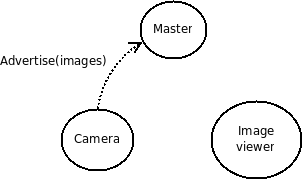
\includegraphics[width=0.30\textwidth]{img/ros_master/ros_master1.png}
    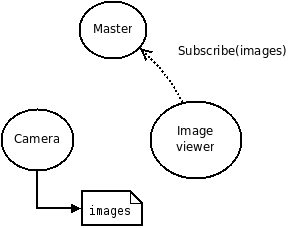
\includegraphics[width=0.30\textwidth]{img/ros_master/ros_master2.png}
    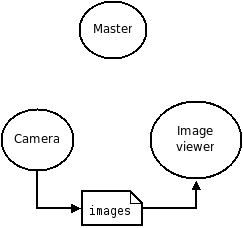
\includegraphics[width=0.30\textwidth]{img/ros_master/ros_master3.png}
    \caption{The process how a camera node informs the ROS-master about the advertisement of information in the images topic and an other image viewer node subscribe to the same topic which leads to a peer-to-peer connection over the images topic.}
    \label{fig:ros_master}
\end{figure}

The advertisement and subscriptions are managed by the ROS-Master which holds the information to establish the peer-to-peer connection.
The first step to establish a successful connection is the notification of the master about the new topic.
To that moment no data is send, because the topic has no subscriber.
To use the information an other node needs to subscribe to the topic by informing the master about the subscription.
Now the master gives the information to establish a peer-to-peer connection between the nodes and the information goes directly from one node to the other.
Figure \ref{fig:ros_master} visualizes the process with an example how a camera node and image viewer node establish their connection \cite{rosMaster}.

The exchanged information are structured in messages which have predefined structures.
ROS provides messages for the most common usages but they can also be custom made.
Each topic is strongly related to a message type, even if the type is not checked by the ROS-master.

\begin{wrapfigure}[10]{O}{0.4\textwidth}
    \centering
    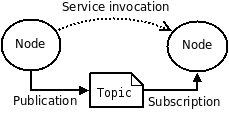
\includegraphics[width=0.4\textwidth]{img/ros_master/service.png}

    \caption{A service invocation is not related to a topic and usually is not a constant flow of messages}
    \label{fig:service_invocation}
\end{wrapfigure}

The publish/subscribe model supports a very flexible way to communicate and can easily scale to big many-to-many models.
But for request/reply situations it is not appropriated.
In these situations services can be used.
They are defined by a pair of messages, one for the request and one for reply.
The call of a service is similar to the connection with a topic except that it is just for the time between the request and the reply.
But nodes can also establish a persistent connection to a service, which causes less robustness but a higher performance.

\subsection{Visualization}\label{ssec:visualization}

In ROS the visualization of data is realized in the tool named RVIZ.
To the user RVIZ itself acts as a host application for different plugins where each message type has it's own plugin.
For ROS RVIZ acts as a normal node so that the individual plugins needs to be configured to subscribe to the relevant topics and how the visualization should look like.

RVIZ provides a number of plugins for the standard messages, but one can also develop their own plugins to visualize the custom messages.

\subsection{Data Recording}\label{ssec:dataRecording}

The ability to record and playback data is a crucial part of ROS.
Since all available data in ROS are exchanged via topics one just needs to subscribe to the topics witch holds the data that should be recorded.
The file format to save the records is typical a bag.
A bag is created with a tool like rosbag.
The tool subscribes to the wanted topics and writes the messages into the bag file, as they come.
After finishing the recording a bag file can be palyed back with the same tool.
For the rest of the ROS network it behaves like the messages are published by the original nodes, which makes the handling very easy.

To make the process of writing and reading into bag files efficient the messages are not saved as messages but in the same representation as in the network transport layer.
To have the ability to invest \ac{ROS} bags without installing \ac{ROS}, a programmatic API is provided to iterate over the messages in a \ac{ROS} bag \cite{rosBag}.


\section{MATLAB}\label{sec:matlab}
MATLAB stands for Matrix Laboratory and is a computing environment with it's own programming language.
It's originally designed by Cleve Moler to give his students easy access to LINPACK and EISPACK which are Fortran packages to solve Eigensystem and Linear Equation problems.
Later it got rewritten and extended in C from Jack Little and Steve Bangert.
The main extensions where functions, toolboxes and graphics.

Today it is developed and distributed by MathWorks, which is founded by Moler, Little and Bangert.
Over the time the number of toolboxes, tools and features increased.
So did the number of users in universities.

Together with Simulink, which is an other product from MathWorks, MATLAB is used at over 5000 universities and can be termed as the engineers language \cite{introductionMatlab}.

\subsection{ROS Toolbox}\label{ssec:rosToolbox}
The \ac{ROS} toolbox is the interface to \ac{ROS} for MATLAB and Simulink and provides the possibilities to create nodes and process the messages from a \ac{ROS} network.
It also provides functions to read from \ac{ROS} bags and handling standard message types.


	\chapter{Realization}\label{ch:realization}

In this chapter it will be described how the used components (chapter\ref{ch:usedComponents}) are combined to create a software environment for mobile thermal mapping solutions.

\section{Software Deployment}\label{ch:realization:sec:softwareDeployment}

We installed \ac{ROS} Melodic Morenia with the package manager of Ubuntu, because it was the long term supported distribution to the time of the research.
But the most third party \ac{ROS} nodes can be found on \href{https://github.com}{Github.com} or directly at the vendors webpage and needs to be installed manually.

The vendors of our sensors provide a \ac{ROS} node for their sensors so that we only need to install drivers and build the \ac{ROS} nodes.
To this moment, we can collect the measurements from the sensors and can access them from one \ac{ROS} network but each node needs to be started individually and on every new installation could have another version of driver or \ac{ROS} node.

To tackle the problems of different versions we created a structure of repositories where each repository holds a specific part and the main repository includes the other repositories.
The modular approach makes it possible to exchange a single sensor and freeze the software version of the node by cloning the repository from the vendor into a own repository.
The main repository also holds scripts to install the drivers.
Also launch files for different operations in the main repository makes is easier to start the ROS system with only one command.
All repositories are published on Github. \todo{add git hub link}

\section{Data Acquisition}\label{ch:realization:sec:dataAcquisition}

After starting the \ac{ROS} project the single nodes use the sensor drivers to collect the data.
They use the predefined messages to prepare the measurements for publishing them and register the topics at the current ROS-Master. \todo{include graph}
As one can see on the node graph the topics of one sensor are merged in meta topics.
With these meta topics it's easier to distinguish between similar topics from different sensors. \todo{Können die wie normale topics gehandhabt werden?}

\subsection{Storing Data}\label{ch:realization:ssec:storingData}

To store data \ac{ROS} provides the ROS bag file format which is described in Chapter~\ref{sec:ros}.
Because we use different cameras which publish a lot of images the bags size increases very fast.
To avoid a long download times the bags should not be stored inside the main repository.
A special repository got created for handling big files which can be used if some old recordings should be used.

To subscribe topics and save the messages we use the \texttt{rosbag} commandline tool.
We tell \texttt{rosbag} which topics to subscribe and save to the bag file with commandline parameter.

Considering the size of the bags and that some file systems like FAT32 can only handle files with a maximum size of 4GB the bag size should not exceed 4GB\@.
This can be archived by an other parameter called \texttt{--split} and \texttt{--size} which specifies the maximum size of one file.
Once a bag file reaches the maximum another bag file gets created.
Each of the bag files can be handled as a independent record so that one can just use the specific file which holds a special scenario.

To have similar, reusable and exchangeable bag files it is a good practice to write a script for the recording.
In this script all parameter are specified together with all topics.
So it only needs to specify the name of the bag file and the script will do everything to record the data.
This script is located in the rosbag-repository to have an easy access.

\subsection{Visualization}\label{ch:realization:ssec:visualization}

In our case the visualization should only give the students an idea how the date looks like.
It does not claim to be perfect accurate in terms of calibration between the different sensors.

\texttt{RVIZ} is used to visualize the messages coming from the sensor nodes.
So we configured the plugins to subscribe to the relevant topics and how the data should be visualized.

Because all measurements are collected in it's own coordinate frame a connection between all frames need to be published to the \texttt{\textbackslash tf} topic.
As a base how to connect the single frames we follow the principles defined in the REF 105~\cite{rosFrames} which makes it simple to combine multiple mobile mapping platforms in one ROS system.
As defined in REF 105 all sensor frames are based on the \texttt{base\_link} and the \texttt{base\_link} is a child of \texttt{odom} and that again is a child of \texttt{map}.

The Static transformation between \texttt{base\_link} and the sensors can be publish with a standard node by calling the node in a \texttt{.launch} file with the transformation parameter as parameter for the node. \todo{add simple frames without sensors img}
The same applies for the transformation between the \texttt{map} and \texttt{odom} frame.
But the transformation between \texttt{odom} and \texttt{base\_link} frame is a dynamic transformation which represents the movement of the whole mobile mapping platform in the \texttt{odom} frame.
So it depends on the measurements of the used IMU\@.

To calculate and publish the transformation a ROS node called "robot\_localization" is used.
This is an implementation of an extended kalmanfilter as ROS node which is open source and published under the BSD license by Charles River Analytics, Inc.
We included the node in the same way like we included the sensor nodes and cloned the repository in sub repository where we can control updates.
This node takes the measurements of the IMU and calculates the new transformation which is then published to the \texttt{\textbackslash tf} topic as transformation from the \texttt{odom} to the \texttt{base\_link} frame.
The implementation is further discussed in the Proceedings of the 13th International Conference on Intelligent Autonomous Systems (IAS-13) by T. Moore and D. Stouch \cite{MooreStouchKeneralizedEkf2014}.

To colorize the pointcloud with the image from the thermal camera the thermal image needs the same resolution as the depth image.
That is archived by a ROS node which subscribes to the image topic from the thermal camera, adds a white border and publish the new image to a new topic.
This new topic can be subscribed by \texttt{RVIZ} to colorize the point cloud.
The size of the white border adjusted in the node and needs to be re-adjusted every time the observed scene changes.

\section{Data Processing}\label{ch:realization:sec:dataProcessing}

Processing data from mobile mapping platform in the context of teaching mostly means to demonstrate algorithm or giving students the option to implement the taught algorithm.
We use MATLAB and the ROS toolbox as environment to provide a simple but also very flexible interface to ROS.
Using MATLAB has the advantage that almost every student and scientist already know the programming language and that it supports all common operating systems.

\subsection{Online}\label{ch:realization:ssec:online}

The online processing is done by writing a node which subscribes to the different topics.
The repository dedicated for data processing contains a template node to provide a uncomplicated start for new contributer or students.

\subsection{Offline}\label{ch:realization:ssec:offline}

To process the recorded measurements offline we developed a MATLAB application to select the bag file, topics output directory and time of the messages which should be extracted.
The MATLAB application provides a graphical interface build with the MATLAB App Designer and can be installed within MATLAB.
We developed the application as a modular system which which provides an interface to use it in other projects.
This can be used by including the related repository into the MATLAB path.

The application take advantage of the selects the topics which are chosen from the user and saves the last message published at the user given time.
The messages are saved as \texttt{*.mat} files in the output directory and collected in a cell array which is returned.

	\chapter{Results}
\section{Visualization}
\section{Data acquisition}

	\chapter{Discussion and Outlook}\label{ch:discussionAndOutlook}

	\appendix

\chapter{Appendix chapter}\label{ch:appendix1}
Lorem ipsum dolor sit amet, consetetur sadipscing elitr, sed diam nonumy eirmod tempor invidunt ut labore et dolore magna aliquyam erat, sed diam voluptua. At vero eos et accusam et justo duo dolores et ea rebum. Stet clita kasd gubergren, no sea takimata sanctus est Lorem ipsum dolor sit amet. Lorem ipsum dolor sit amet, consetetur sadipscing elitr, sed diam nonumy eirmod tempor invidunt ut labore et dolore magna aliquyam erat, sed diam voluptua. At vero eos et accusam et justo duo dolores et ea rebum. Stet clita kasd gubergren, no sea takimata sanctus est Lorem ipsum dolor sit amet.

	% references
	\bibliography{./bib/literature}
\end{document}
